\documentclass[letterpaper]{article}
 \usepackage{float}
 \usepackage[margin=2.54cm]{geometry}
 \usepackage{graphicx}
 \usepackage{anysize}
 \usepackage{lipsum}
 \usepackage{amsmath,amssymb,amsthm}
 \usepackage[utf8]{inputenc}
 \usepackage{multirow}
 \usepackage{csquotes}
 \usepackage[spanish]{babel}
 \usepackage{apacite}
 \usepackage{multicol}
 \usepackage{parskip}
 \usepackage{setspace} 
\usepackage{empheq}
\usepackage{mdframed}
\usepackage{booktabs}
\usepackage{lipsum}
\usepackage{graphicx}
\usepackage{color}
\usepackage{psfrag}
\usepackage{pgfplots}
\usepackage{bm}
\usepackage{tocloft}
\geometry{letterpaper, margin=2.54cm}
\begin{document} 
\pgfplotsset{compat=1.18}
\setstretch{2}
\begin{titlepage}
	\centering
	\vspace{3cm}
	{\scshape\Huge Trabajo de Mecánica de Fluidos \par}
	\vspace{3cm}
	\textbf\large\scshape{\par}
	\vspace{3cm}
	{\Large Vergara Pareja Gustavo\\Valdéz Godin Aldair\\Pila Mendoza José\par}
	\vspace{4cm}
	{\scshape\Large Programa de Ingeniería Mecánica \par}
	{\scshape\Large Universidad de Córdoba\par}
	{\Large \today \par}
\end{titlepage}
\tableofcontents
\newpage
\section{Introducción}
%\%contentsline{toc}{section}{Introducción}
El presente proyecto tiene como objetivo principal aplicar los principios de flotabilidad y estabilidad 
en el diseño y construcción de un bote. La mecánica de fluidos es una rama fundamental de la física que 
estudia el comportamiento de los fluidos en reposo o en movimiento. En este caso, nos enfocaremos en la 
forma en que los fluidos interactúan con el bote y cómo se puede lograr que este flote y se mantenga 
estable en el agua.
\newline

Se responderán preguntas
como: ¿Cómo se diseñó el casco?, ¿Con qué materiales se construyó? y ¿Cuál es su finalidad?.
\newline
Para lograr este objetivo, se utilizarán principios de la física y la mecánica para describir
el movimiento del casco y se analizarán las fuerzas involucradas en su funcionamiento.
Además, se describirá el diseño mecánico de este, incluyendo los materiales utilizados
y las especificaciones técnicas.
\newpage
\section{Objetivos}
%contentsline{toc}{section}{Objetivos}
\subsubsection{Objetivo General}
\begin{itemize}
	\item Diseñar y construir el casco de un bote aplicando los principios de flotabilidad y estabilidad.
\end{itemize}
\subsubsection{Objetivos Específicos}
\begin{itemize}
	\item Analizar y aplicar los conceptos teóricos de la mecánica de fluidos para comprender los principios de flotabilidad y estabilidad en el diseño de embarcaciones.
	\item Diseñar un bote que cumpla con los criterios de flotabilidad y estabilidad, considerando la ubicación del centro de gravedad, el centro de flotación y la forma del casco.
	\item Evaluar experimentalmente el desempeño del bote en términos de flotabilidad y estabilidad, realizando pruebas en condiciones controladas de agua y registrando datos relevantes como la inclinación, el desplazamiento y la capacidad de carga del bote.
\end{itemize}
\newpage

\section{Teoría Relacionada}
%contentsline{toc}{section}{Teoría Relacionada}
\subsubsection{Hidrostática}
\setlength{\parindent}{18pt}

El término hidrostática se refiere al estudio de los fluidos en reposo.

\subsubsection{Fluido}
\setlength{\parindent}{18pt}
Un fluido es una sustancia que se deforma continuamente cuando es sometida 
a un esfuerzo cortante, no importa si el esfuerzo cortante es muy pequeño. (Streter y Wylie 1991, p.3). 

\subsubsection{Principio de Arquímedes}
\setlength{\parindent}{18pt}
Se conoce que los barcos flotan, gracias a los aportes realizados por el físico Arquímedes;
La fuerza de flotación que actúa sobre un cuerpo sumergido en un fluido es igual
al peso del fluido desplazado por el cuerpo y actúa hacia arriba pasando por el
centroide del volumen desplazado. Para los cuerpos flotantes, el peso del cuerpo completo debe ser igual a la fuerza
de flotación ($F_{e}$), la cual es el peso del fluido ($W$) cuyo volumen es igual al de la parte sumergida
de ese cuerpo, (Cengel and Cimbala 2018, p.101). 
\begin{equation}
	F_{e}= W = \gamma \cdot  V_{sum} 
\end{equation}

\subsubsection{Centro de gravedad}
\setlength{\parindent}{18pt}
La resultante de las fuerzas de gravedad que actúan sobre un cuerpo, el cual conocemos
como el peso del cuerpo, actúa por un punto denominado centro de gravedad
del cuerpo. El centro de gravedad entonces se determina por la distribución del peso
dentro del cuerpo, (Pytel 2009, p.442).

\subsubsection{Metacentro}
\setlength{\parindent}{18pt}
El metacentro (mc) se define como
la intersección del eje vertical de un cuerpo cuando está en su posición de equilibrio,
con una línea vertical que pasa a través de la posición nueva del centro de flotación
cuando el cuerpo gira levemente.
\begin{figure}[H]
	\centering
	\includegraphics[width=0.6 \textwidth]{Metacentro.png}
	\caption{ Posición del metacentro. Mott, (2006)}
	\label{fig:imagen0}
\end{figure}
Donde:
\newline
\textbf{cg}, es el centro de gravedad.
\newline
\textbf{cb}, es el centro geométrico de la carena sumergida.
\newline
\textbf{mc}, es el punto de cruce de la línea vertical del centro del cuerpo con el plano de la línea central, 
conocido como Metacentro.


Si \textbf{mc} se sitúa arriba del centro de gravedad, el cuerpo es estable (Mott 2006, p.135).

\subsubsection{Estabilidad}
\setlength{\parindent}{18pt}
``La estabilidad se refiere a la
capacidad que tiene un cuerpo
de regresar a su posición original
después de inclinarse con
respecto de un eje horizontal. La condición de estabilidad para los cuerpos sumergidos por completo en un
fluido es que su centro de gravedad esté por debajo de su centro de flotabilidad'', (Mott 2006 p.133).
\subsubsection{Flotabilidad}
\setlength{\parindent}{18pt}
``La flotabilidad se define como aquella capacidad que posee un cuerpo para sostenerse dentro de un fluido, 
donde la fuerza flotación actúa en dirección vertical hacia arriba a través del centroide del volumen 
desplazado'', (Mott 2006, p.124).
\subsubsection{Casco de deplazamiento}
\setlength{\parindent}{18pt}
``Es el cuerpo de una embarcación, sin contar los elementos móviles como: 
superestructuras, máquinas, arboladura, pertrechos (recambios), etc.'' (Escola Port Aula Náutica, 2022).
\subsubsection{Dimensiones del Barco}
\setlength{\parindent}{18pt}
Para cualquier diseño de una embarcación que se desea analizar, es necesario conocer cada parte de esta 
estructura ingenieril. Las dimensiones principales que conforman un barco son, eslora máxima, es la longitud 
total del casco, la cual comprende desde la proa hasta la popa, manga máxima, es la mayor anchura de la 
cuaderna con estructuras asentadas, el calado, es la distancia desde la parte inferior de la quilla a la 
línea de flotación, el puntal, es la distancia máxima vertical medida desde la quilla hasta cubierta 
principal, la escora, es el ángulo de inclinación lateral de la embarcación y el asiento, es la diferencia
 en inclinación entre los calados de popa y de proa, esta se clasifica en apopante, 
 apropante y neutro o sentado. (Benítez y Silva 2023, p.5).
 \begin{figure}[h]
	\centering
	\includegraphics[width=0.8 \textwidth]{dimensionestemporal.jpg}
	\caption{ Dimensiones de un barco}
	\label{fig:imagen00}
\end{figure}
\newpage
\section{Materiales y máquinas}
%contentsline{toc}{section}{Materiales y métodos}
Los materiales utilizados para el desarrollo de este casco fueron:
\begin{itemize}
	\item Madera (Roble)
	\item Pintura
	\item Marcadores
	\item Cincel
	\item Martillo
	\item Lápiz
	\item Escuadra
	\item Sierra circular
	\item Lijas
	\item Pulidora
\end{itemize}

\newpage
\section{Contenido y Resultados}
%contentsline{toc}{section}{Contenido y Resultados}
El objetivo de este proyecto fué estudiar el movimiento del casco de un bote y realizar cálculos empíricos
de su flotabilidad, estabilidad y análisis de fuerzas. Para el diseño, se construyó el casco de un barco 
a escala, y luego se realizaron pruebas en condiciones controladas de agua.
Para el desarrollo de este proyecto, hicimos una búsqueda exhaustiva de modelos e ideas para construir el casco del barco.
\begin{figure}[H]
	\centering
	\includegraphics[width=0.7\textwidth]{planosbarc.png}
	\caption{ Planos oficiales ClassGlobe 5.80.}
	\label{fig:imagen}
\end{figure}
\begin{itemize}
	\item A continuación, tomamos el diseño y las relaciones de medidas, y comenzamos a diseñar el casco de nuestro barco.
\end{itemize}
\begin{figure}[H]
	\centering
	\includegraphics[width=0.7\textwidth]{Cascobarco.png}
	\caption{Plano del casco en Autocad}
	\label{fig:imagen1}
\end{figure}
\begin{itemize}
	\item Con ayuda de herramientas de carpinteria y la supervision de expertos, logramos un excelente producto final.
\end{itemize}
\begin{figure}[H]
	\centering
	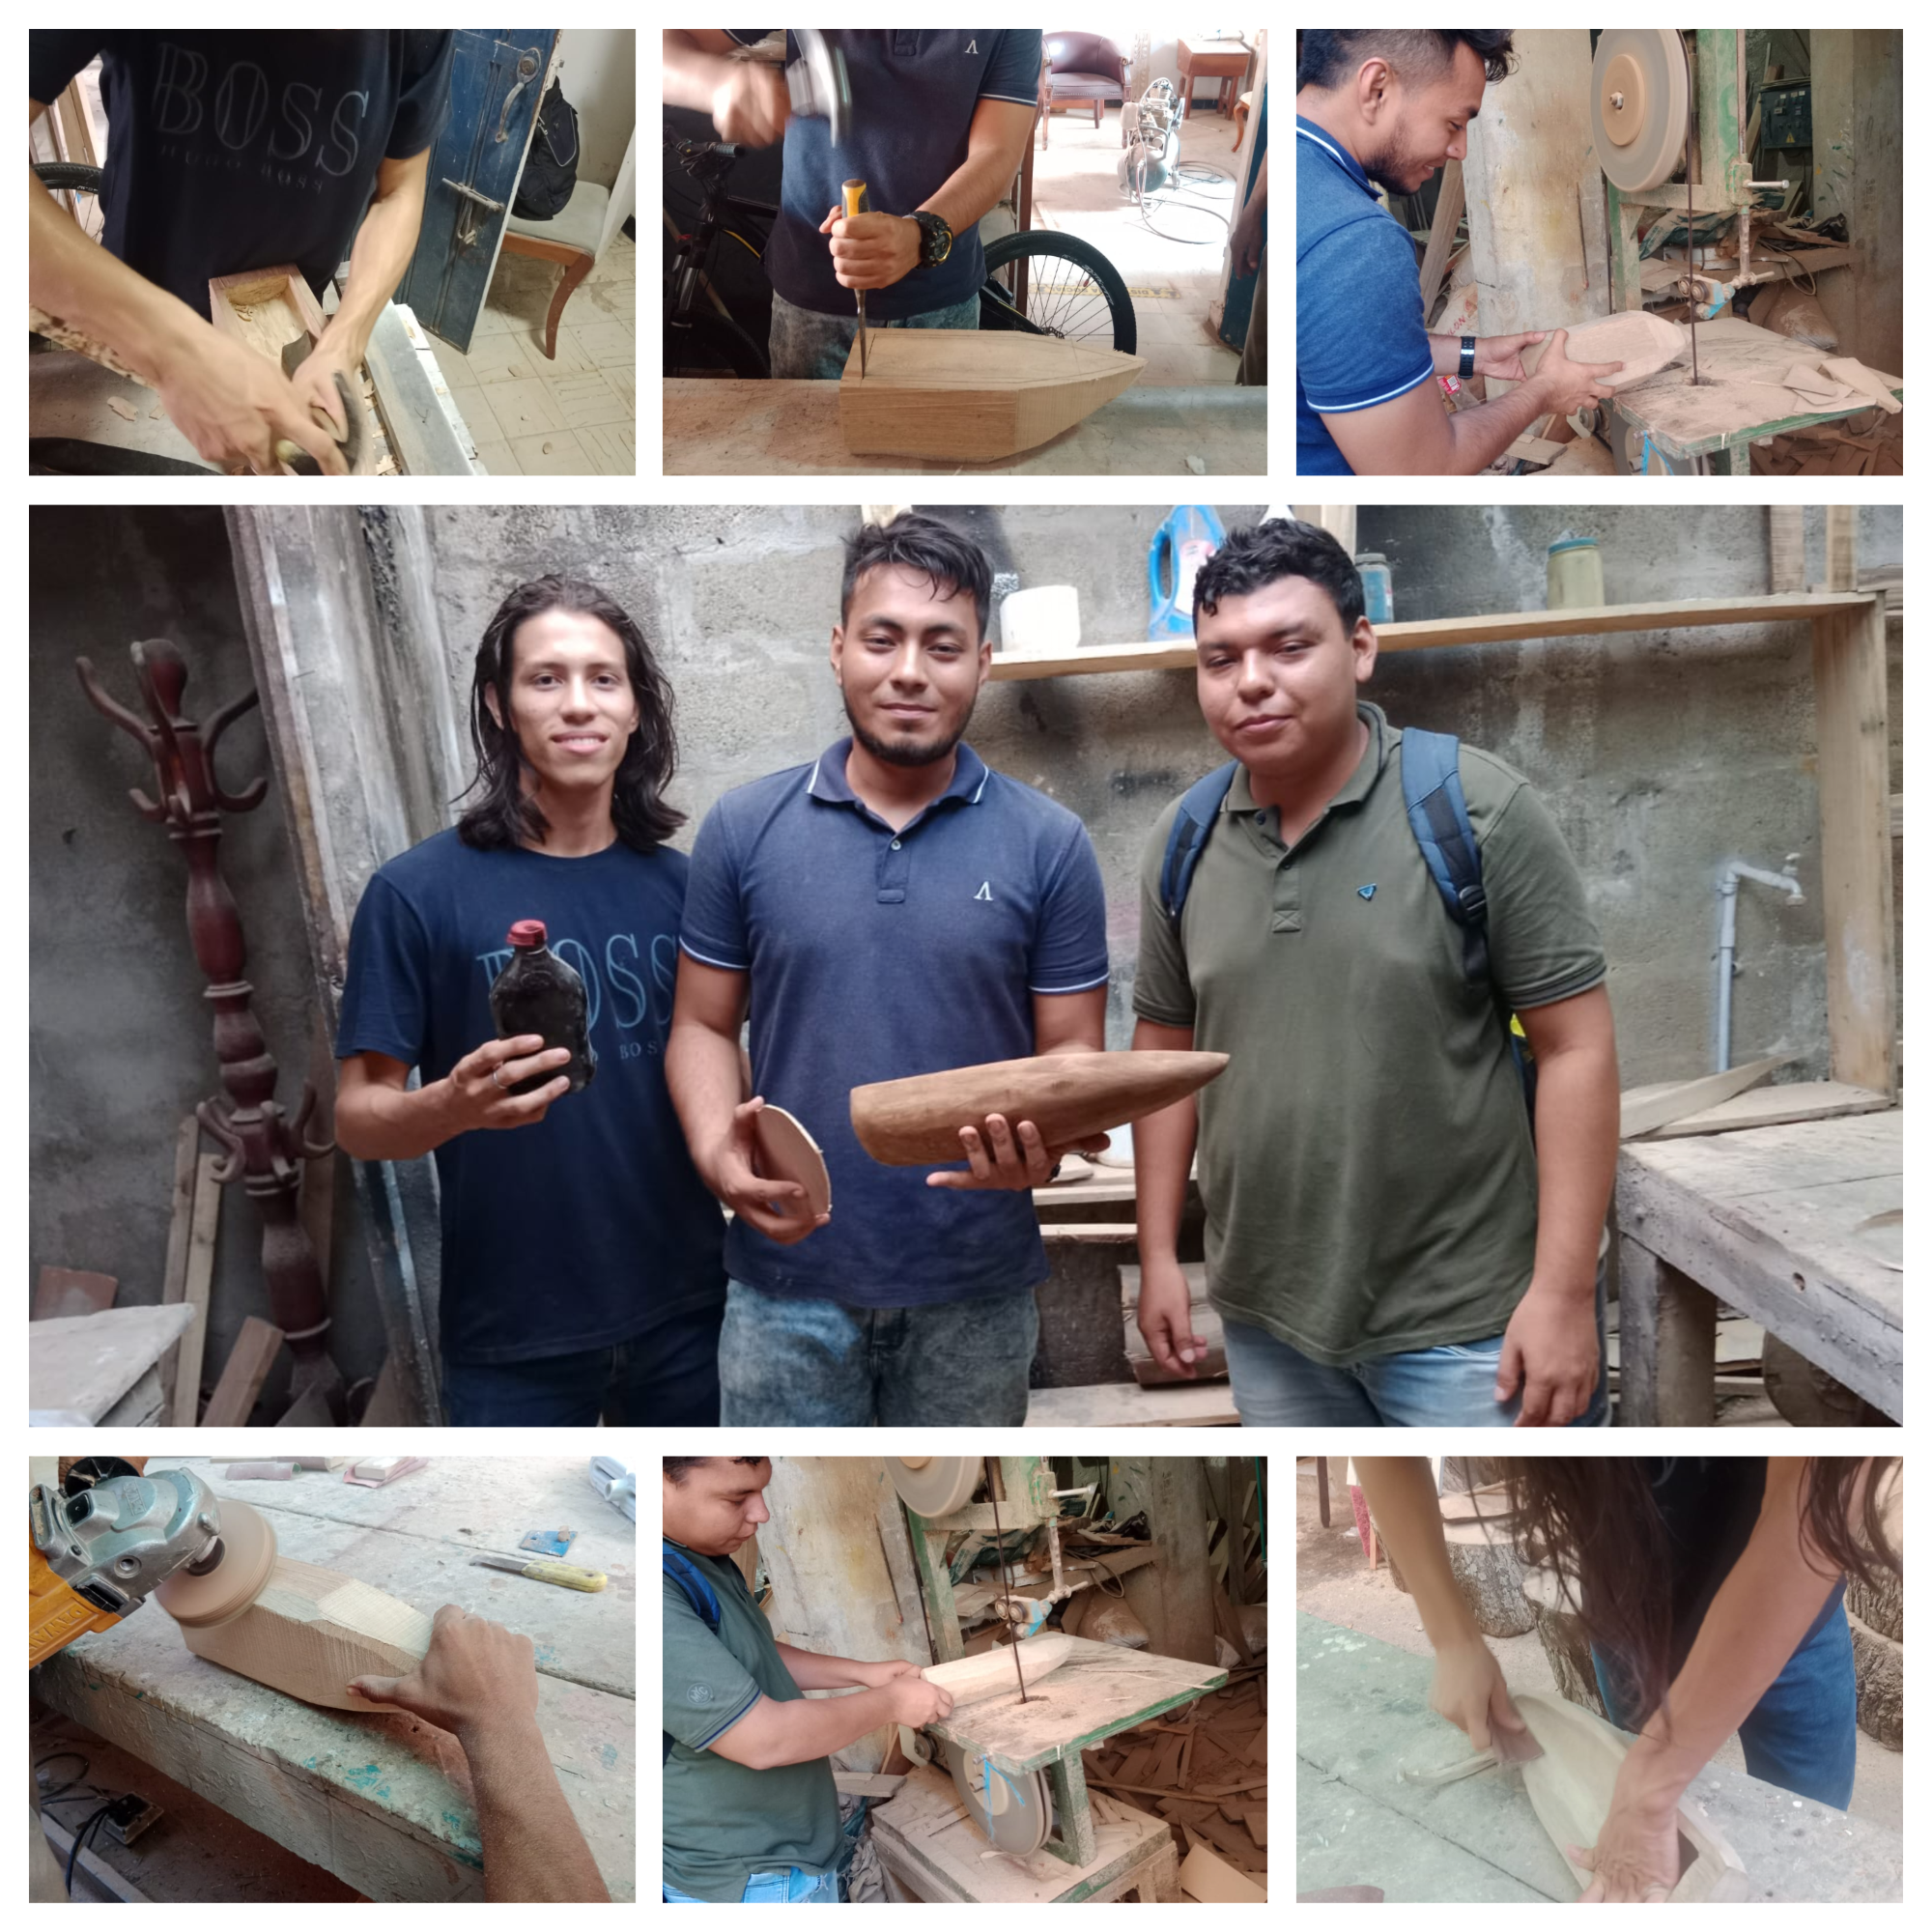
\includegraphics[width=1\textwidth]{Collage1.png}
	\caption{Fases de la construcción y producto final}
	\label{fig:imagen2}
\end{figure}
\newpage
%\begin{itemize}
	%\item Análisis del barco
%\end{itemize}
%\begin{figure}[H]
	%\centering
	%\includegraphics[width=0.8\textwidth]{imgbarcofinal.png}
	%\caption{Carga máxima, centro de gravedad y flotabilidad\ldots}
	%\label{fig:imagen3}
%\end{figure}
%\newpage
A continuación, se presenta el análisis hidrostático del barco; El cual tiene dos momentos uno con el barco sin peso y otro con peso:
\newline
Ahora, definimos algunas propiedades del barco:
\begin{equation}
	\rho_{roble}=\frac{m_{barco}}{V_{barco}} \rightarrow {V_{barco}}=\frac{ m_{barco}} {\rho_{roble}}
\end{equation}

\begin{equation}
	 {V_{barco}}=\frac{ 815g} {0,8 \cdot g/cm^3} = 1018,75 cm^3
\end{equation}
\subsection{Línea de Flotabilidad}
Ahora bien, sabiendo que $W$=$F_b$; 
\begin{equation}
	L_{sum}=\frac{{V_{barco}} \cdot \rho_{roble}}{0,4~cm \cdot 0,12~cm \cdot \rho_{agua}}=\frac{{1018,75~cm^3} \cdot 0.8g/cm^3}{360~cm^2 \cdot 1g/~cm^3}=2,20~cm
\end{equation}
Por lo tanto la línea de flotabilidad se encuentra a 2,20 cm desde el fondo del barco.
\subsection{Centro de flotación}
EL centro de flotación será el centro de gravedad del volumen desplazado.
\newline
\hspace{0.5cm}$V_{d}=V_{sum}$;
\begin{equation}
	V_{sum}= \frac{(\pi \cdot ab)*27~cm}{2} = \frac{(\pi \cdot 2,2cm \cdot 6cm)*27~cm}{2} = 560~cm^3
\end{equation}
$C_{b}$ = Centroide de la carena sumergida.
La carena sumergida tiene la forma de media elipse; Así entonces,:
$\bar{x}=a = 5~cm$;
\newline 
$\bar{y}= \frac{4b}{3\pi} = \frac{4(2,2cm)}{3\pi} = 0,934cm$
\newline
Así entonces, el centro de flotación se ubica 0,934 cm desde el fondo del barco.
\newpage 
\subsection{Centro de gravedad}
$C_{g}$ = Centro de gravedad de la figura.
\newline
$\bar{x}=0 cm$;
\newline 
$\bar{y}= \frac{4r}{3\pi} = \frac{4(6cm)}{3\pi} = 2,55~cm$
Así entonces, el centro de gravedad se ubica 2,55 cm desde el fondo del barco.
\subsection{Metacentro}
$M_{c}$ = $C_{b}$ + $MB$
\newline
\begin{equation}
	MB=\frac{I_{c}}{V_{d}} = [\frac{(20~cm \cdot 12~cm^3)}{12} + \frac{(20~cm \cdot 12~cm^3)}{36}] \cdot \frac{1}{1018,75cm^3} = 3,769~cm
\end{equation}
\begin{equation}
	M_{c} = C_{b} + MB = 4,7cm
\end{equation}
\newline
Así entonces, el Metacentro se ubica 4,7 cm desde el fondo del barco.
\newline
Todos estos calculos fueron realizados sin la masa de 300g sobre el barco.
A continuacion se realizarian los mismos calculos pero con la masa de 300g sobre el casco, el procedimiento es el mismo y los datos estimados son:
\newline
\begin{itemize}
	\item La línea de flotabilidad se encuentra a  3,1 cm desde el fondo del barco.
	\item El centro de flotación se ubica 4,68 cm desde el fondo del barco.
	\item El centro de gravedad se ubica 3,45 cm desde el fondo del barco.
	\item El Metacentro se ubica 5,09 cm desde el fondo del barco.
\end{itemize}
		

\section{Conclusiones}
%contentsline{toc}{section}{Conclusiones}
En conclusión, el proyecto de diseño y construcción de un bote basado en los principios de flotabilidad y estabilidad es una oportunidad para aplicar los conocimientos teóricos de la mecánica de fluidos de manera práctica y significativa. A lo largo del proyecto, se han abordado conceptos clave como el principio de Arquímedes, el centro de flotación y la estabilidad.
El diseño y construcción de un bote que cumpla con los principios mencionados requiere un enfoque integral que considere tanto los aspectos teóricos como los prácticos. Las dificultades enfrentadas se presentaron al momento de construirlo. El diseño se compone de cortes complejos, y hacer los cortes perfectos es un trabajo muy difícil, tales imperfecciones afectaron la precisión de los calculos. Se han explorado conceptos teóricos fundamentales y se han aplicado en la práctica a través de la construcción del bote y la evaluación experimental de su desempeño en términos de flotabilidad y estabilidad.
Este proyecto ha permitido comprender la relación entre la teoría de la mecánica de fluidos y su aplicación práctica en el diseño y construcción de embarcaciones. Estos conocimientos adquiridos son valiosos tanto en el ámbito académico como en el profesional, ya que la mecánica de fluidos juega un papel fundamental en numerosas disciplinas relacionadas con el diseño.


\newpage
\section*{}
\bibliographystyle{apacite}
\nocite{*}
\bibliography{referenciados}
\end{document}